% This text is proprietary.
% It's a part of presentation made by myself.
% It may not used commercial.
% The noncommercial use such as private and study is free
% Sep. 2005
% Author: Sascha Frank
% University Freiburg
% www.informatik.uni-freiburg.de/~frank/


\documentclass{beamer}
\usepackage{graphicx}

%%%%%%%%%%%%%%%%%%%%%%%%%%%%MACROS

\def\var#1{\mbox{\textrm{\bf{\sc{#1}}}}}
\newcommand{\set}[1]{\{#1\}}
\newcommand{\V}{\mathbb{V}}
\newcommand{\E}{\mathbb{E}}
\newcommand{\size}[1]{\ensuremath{\left|#1\right|}}

\newcommand {\framedgraphic}[3] {
    \frame{\frametitle{#1}
        \begin{center}
            \includegraphics[width=\textwidth,height=#3\textheight,keepaspectratio]{#2}
        \end{center}
    }
}
\newcommand{\disableframe}[1]{}

\def\func#1#2{\mbox{\textrm{\bf{\sc{#1}}}}\ensuremath{({#2})}}
% pseudocode notations
\newcommand{\T}{\mbox{\hspace{0.5cm}}}

% asymptotic notations
\newcommand{\Oh}[1]{\ensuremath{{\mathcal O}\left({#1}\right)}}
\newcommand{\Om}[1]{\ensuremath{{\Omega}\left({#1}\right)}}
\newcommand{\Th}[1]{\ensuremath{{\Theta}\left({#1}\right)}}

\newcommand{\ceil}[1]{\ensuremath{\left\lceil#1\right\rceil}}
\newcommand{\floor}[1]{\ensuremath{\left\lfloor#1\right\rfloor}}
\newcommand{\maybepause}{
    \iffalse
    \pause
    \fi
}
\definecolor{light-gray}{gray}{0.35}
\definecolor{orange}{cmyk}{0,0.5,1,0}
\def\comment#1{\hfill{\color{light-gray}{$\left\{\textrm{{{#1}}}\right\}$}}}
\def\lcomment#1{\hfill{\color{light-gray}{$\left\{\textrm{{{#1}}}\right.$}}}
\def\rcomment#1{\hfill{\color{light-gray}{$\left.\textrm{{{#1}}}\right\}$}}}
\def\fcomment#1{\hfill{\color{light-gray}{$\textrm{{{#1}}}$}}}


%%%%%%%%%%%%%%%%%%%%%%%%%%%%MACROS

\setbeamertemplate{footline}[text line]{%
    \parbox{\linewidth}{
        \vspace*{-8pt}
        \hspace*{-20pt}
        \insertshorttitle
        \hfill
        \insertpagenumber
    }
}
\begin{document}
\title[A new optimal algorithm for Level-Synchronous Parallel BFS in the Cilk model]{A new optimal algorithm for Level-Synchronous Parallel BFS in the Cilk model}
\author{Yonatan R. Fogel}
\institute{Stony Brook University}
\date{\today}

\frame{\titlepage}

%TODO: Maybe re-add table of contents
%\frame{\frametitle{Table of contents}\tableofcontents}

\section{Introduction}
\frame{\frametitle{BFS}
    \begin{itemize}
        \item Given
            \begin{itemize}
                \item Graph $G=(\V,\E)$ with diameter $D$ and max out-degree $\Delta$
                \item Source vertex $s \in \V$
            \end{itemize}
        \item Calculate
            \begin{itemize}
                \item $Dist_{u\in \V} =$ length of the shortest path from $s$ to $u$ in $G$
            \end{itemize}

            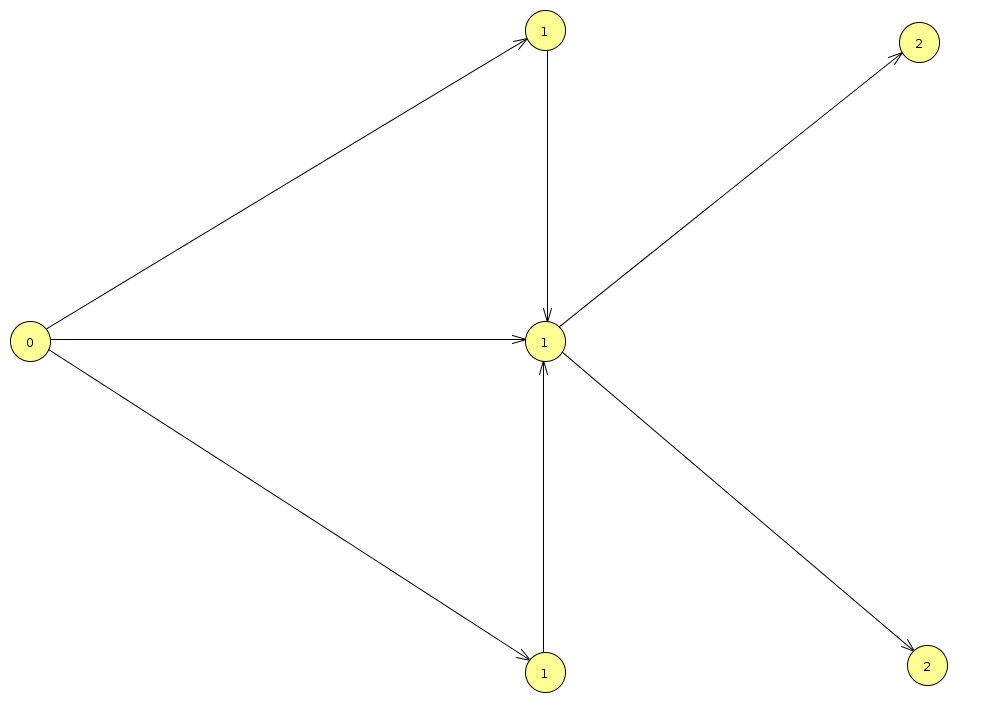
\includegraphics[width=\textwidth,height=0.5\textheight,keepaspectratio]{bfs-1.png}
    \end{itemize}
}

\frame{\frametitle{Parallel BFS}
    \begin{itemize}
        \item The runtime for serial BFS is $T_s=\Th{\size{\V}+\size{\E}}$
        \item For large graphs, calculating $Dist$ can be slow
        \item We can speed up BFS by processing edges and/or nodes in parallel
        \item Our new TBN-BFS achieves near-perfect linear speadup when $p \ll \frac{\size{V}+\size{E}}{D\log\left(\size{V}+\size{E}\right)}$

            \bigskip
            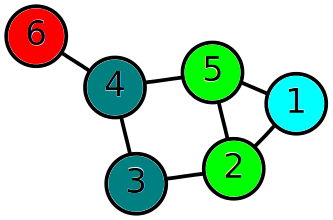
\includegraphics[width=\textwidth,height=0.25\textheight,keepaspectratio]{6n-graf.png}
    \end{itemize}
}

\frame{\frametitle{Level-Synchronous BFS}
    \begin{itemize}
        \item All nodes at distance $d$ from $s$ are processed before any nodes at distance $d^\prime > d$ \maybepause
        \item Level-Synchronous BFS has lower bounds of
            \begin{itemize}
                \item $T_p = \Om{\frac{\size{\V}+\size{\E}}{p}+D}$
                \item $T_1,W_p = \Om{T_s} = \Om{\size{\V}+\size{\E}}$
            \end{itemize}
        \item Non Level-Synchronous BFS algorithms
            \begin{itemize}
                \item Distinguished-BFS \cite{distinguished-bfs}
            \end{itemize}

            \bigskip
            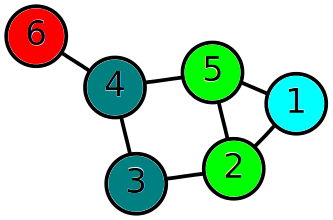
\includegraphics[width=\textwidth,height=0.25\textheight,keepaspectratio]{6n-graf.png}
    \end{itemize}
}

\frame{\frametitle{Cilk Model}
    \begin{itemize}
        \item Large shared memory
        \item Consistent caches between cores
        \item Synchronizing (or launching) $n$ tasks takes $T_\infty=\Th{\log n}$ time
        \item Cilk+ has this model with the addition of randomized work stealing \cite{cilk}
        \item A parallel algorithm has the following properties
            \begin{itemize}
                \item $T_p =$ running time using $p$ cores
                \item $T_1 =$ running time using $1$ core
                \item $W_p =$ work done using $p$ cores
            \end{itemize}

            \bigskip
            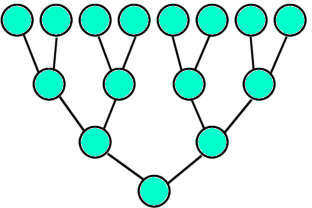
\includegraphics[width=\textwidth,height=0.25\textheight,keepaspectratio]{FullBinary.png}
    \end{itemize}
}

\frame{\frametitle{Non Cilk Model}
    \begin{itemize}
        \item Level Synchronous BFS algorithms not using the Cilk Model
            \begin{itemize}
                \item Cray-BFS uses the Cray MTA-2 hardware model \cite{cray-bfs}
                \item Block-Queue-BFS uses the Intel Mic hardware model \cite{block-queue-bfs}
                \item Blue-BFS uses the BlueGene/L hardware model \cite{blue-bfs}
            \end{itemize}

            \bigskip
            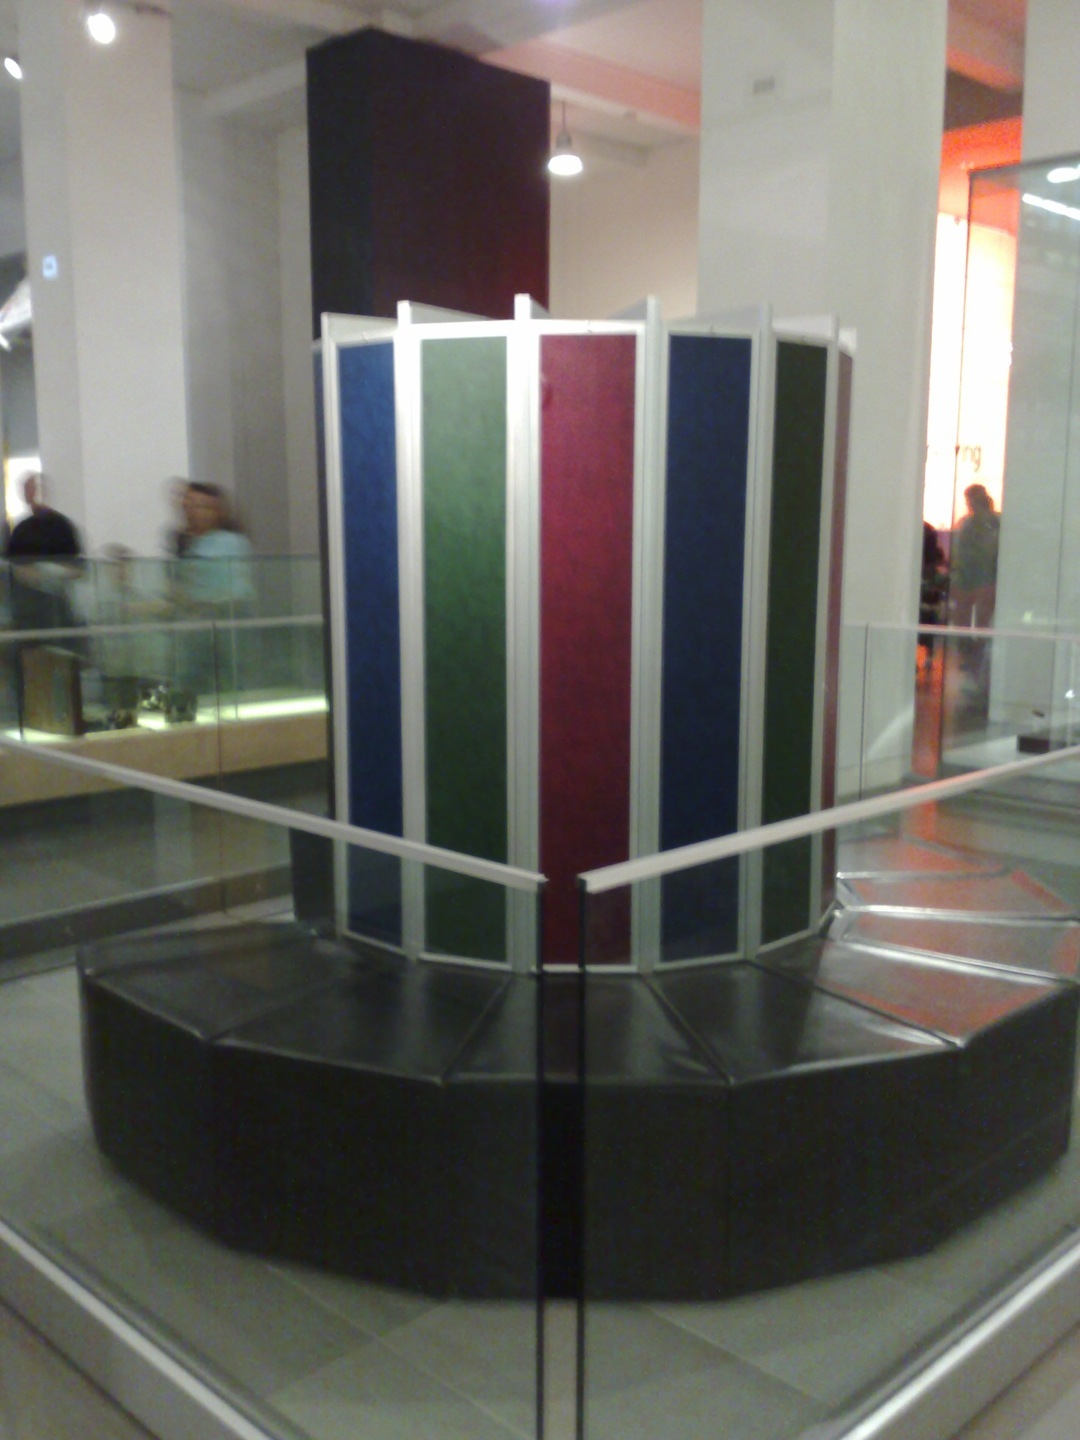
\includegraphics[width=\textwidth,height=0.25\textheight,keepaspectratio]{cray.jpg}
    \end{itemize}
}

\frame{\frametitle{Level-Synchronous Parallel BFS in the Cilk Model}
    \begin{itemize}
        \item In the Cilk Model, Level-Synchronous BFS has a lower bound of $T_p = \Om{\frac{\size{\V}+\size{\E}}{p}+D\log p}$
        \item MIT-Bag-BFS uses penants, bags, and reducer hyperobjects \cite{mit-bag}
        \item Our new TBN-BFS algorithm
            \begin{itemize}
                \item Runs on standard hardware implemented using Cilk+
                \item Can do its own scheduling deterministically
                \item Achieves the lower bound for $T_p, T_1, W_p$ in the worst case independently of $\Delta$ (scale-free)
            \end{itemize}

            \bigskip
            \includegraphics[width=\textwidth,height=0.25\textheight,keepaspectratio]{jet-engine.jpg}
    \end{itemize}
}


\frame{\frametitle{Serial-BFS}
    \begin{enumerate}
        \item for each vertex $u \in \V$
        \item \T $Dist_u \gets \infty$
        \item $Dist_s \gets 0$
        \item $Q \gets \emptyset$
        \item $\func{Enqueue}{Q, s}$
        \item while $Q \neq \emptyset$ do
        \item \T $u \gets \func{Dequeue}{Q}$\label{par1}
            \lcomment{Potential source of\qquad}
        \item \T for each vertex $v$ in $\Gamma(u)$ do\label{par2}
            \rcomment{parallelism: lines \ref{par1}--\ref{par2}}
        \item \T \T if $Dist_v = \infty$ then\label{issue1}
            \lcomment{Potential issues for\qquad}
        \item \T \T \T $Dist_v \gets Dist_u + 1$
            \rcomment{parallelism: lines \ref{issue1}--\ref{issue2}}
        \item \T \T \T $\func{Enqueue}{Q, v}$\label{issue2}
    \end{enumerate}
}

%TODO: Maybe restore this slide (requires edits).  Will probably also require being MOVED ELSEWHERE
%TODO: If I do this, specify what hot topic means (estimate of papers in what conferences over what years)
\disableframe{\frametitle{Motivation for (P)BFS}
    BFS is a hot topic recently and is used for
    \begin{itemize}
        \item Path Finding 
            \begin{itemize}
                \item Video Games
                \item GPS
            \end{itemize}
        \item Analyzing social networks
        \item Designing and analyzing VLSI
        \item Task scheduling
        \item As a primitive in other algorithms
    \end{itemize}
}

\disableframe{\frametitle{Bottlenecks for Parallelizing BFS}
    \begin{itemize}
        \item FIFO
        \item $Dist$ array
    \end{itemize}
}

\section{TBN-BFS}
\frame{\frametitle{TBN-BFS - Summary}
    \begin{itemize}
        \item $T_1 = \Oh{\size{\V}+\size{\E}}$ (optimal)
        \item $W_p = \Oh{\size{\V}+\size{\E}}$ (optimal)
        \item $T_p = \Oh{\frac{\size{\V}+\size{\E}}{p}+D\log p}$ (optimal)
        \item Scale-free
        \item Runs on standard hardware implemented using Cilk+
        \item Can do its own scheduling deterministically

            \bigskip
            
\includegraphics[width=\textwidth,height=0.25\textheight,keepaspectratio]{kitten.jpg}
    \end{itemize}
}

%TODO: no capital in middle (Prepare to Split Work)
\frame{\frametitle{TBN-BFS - High Level}
    \begin{itemize}
        \item To get optimal $T_1,T_p$ the algorithm is
            \begin{enumerate}
                \item For each level $\ell \in [0\ldots D)$
                        \begin{enumerate}
                            \item Prepare to split work
                            \item Split work and process edges
                            \item Deduplicate vertexes and combine queues
                        \end{enumerate}
                \end{enumerate}
            \item To get optimal $W_p$ modify the algorithm to
                \begin{enumerate}
                    \item Reduce search space
                    \item Dynamically choose number of cores
                \end{enumerate}

                \bigskip
                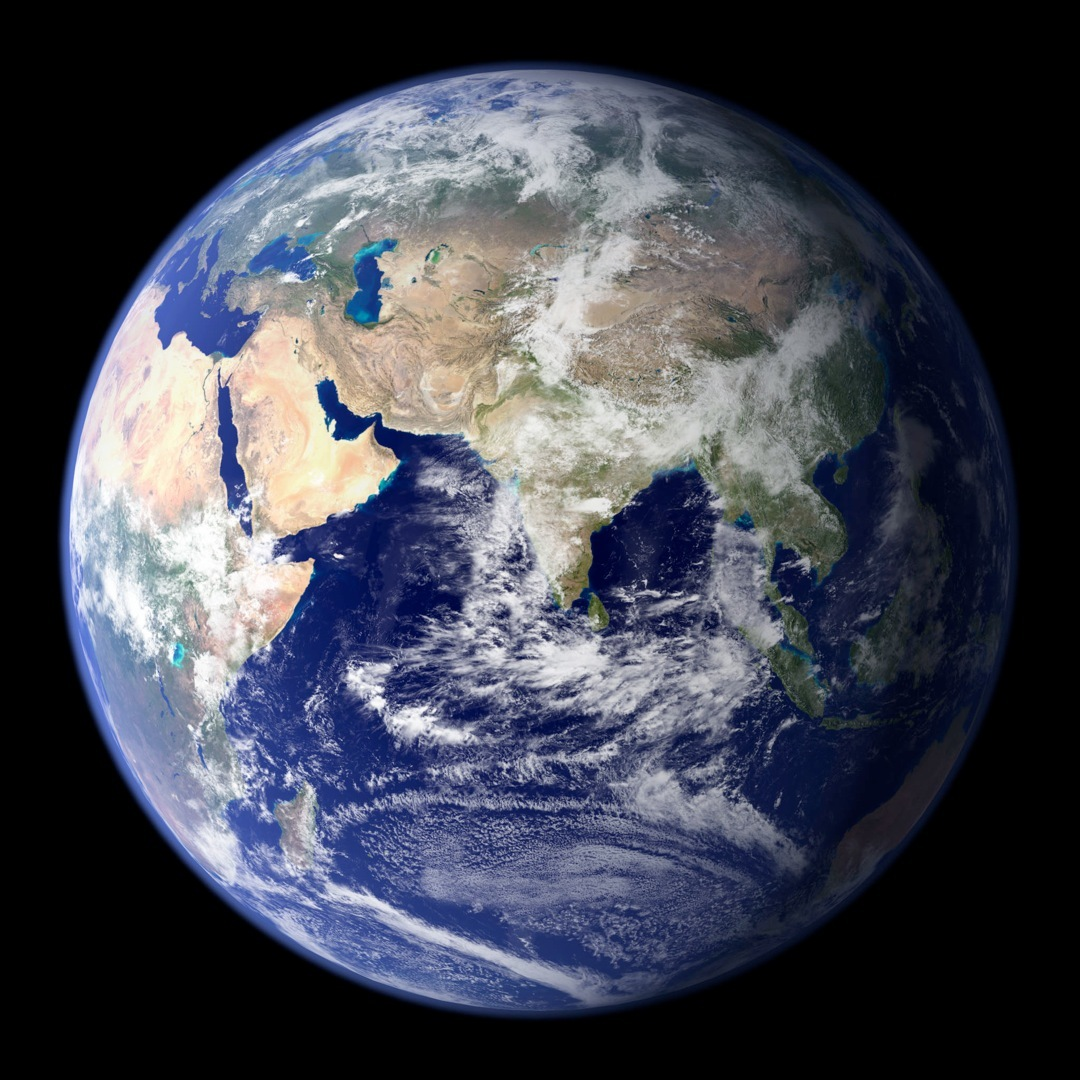
\includegraphics[width=\textwidth,height=0.25\textheight,keepaspectratio]{earth.jpg}
        \end{itemize}
    }

    \subsection{Algorithm}
    \frame{\frametitle{TBN-BFS - Prepare to Split Work}
        \begin{enumerate}
            \item Receive input $Q_{in}\subseteq \V$ where
                \begin{enumerate}
                    \item Each vertex in $Q_{in}$ is unique
                    \item $\forall u \in Q_{in} : Dist_u = \ell$
                    \item $\forall u \in Q_{in} : \size{\Gamma(u)} > 0$
                \end{enumerate}
            \item Generate $OutDegrees[0\leq i<\size{Q_{in}}] = \size{\Gamma(Q_{in}[i])}$ in parallel
            \item Perform a parallel prefix sum on $OutDegrees$
                \begin{tabular}{r|l|l|l|l|l|l|}
                    \cline{2-7}
                    $Q_{in}=$ &1 & 3 & 2 & 4 & $\ldots$ & $\ldots$ \\ \cline{2-7}
      $OutDegrees_{before} =$ &5 & 7 & 1 & 2 & $\ldots$ & $\ldots$ \\ \cline{2-7}
      $OutDegrees_{after}  =$ &5 & 12 & 13 & 15 & $\ldots$ & $m_\ell$ \\ \cline{2-7}
                \end{tabular}
        \end{enumerate}

                \bigskip
                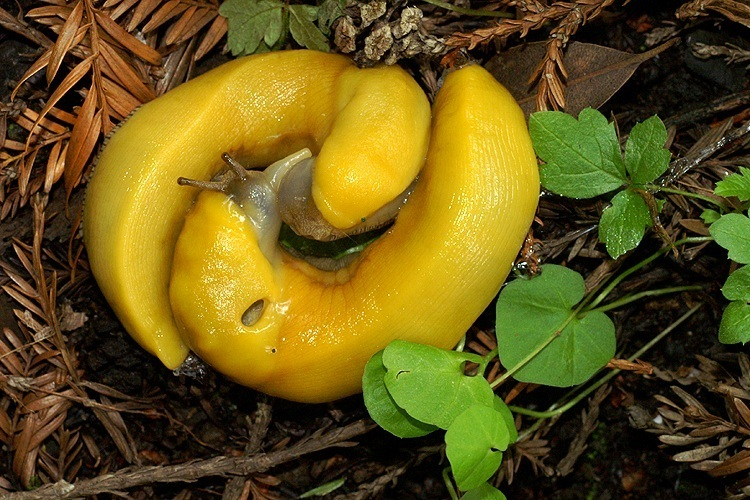
\includegraphics[width=\textwidth,height=0.25\textheight,keepaspectratio]{banana.jpg}
    }

    %TODO: Maybe add a picture? (WHAT?)
    \frame{\frametitle{TBN-BFS - Split Work and Process Edges}
        \begin{enumerate}
            \item Each core $i$ in parallel
                \begin{enumerate}
                    \item searches $OutDegrees$ for $1+\floor{\frac{i ~ m_\ell}{p}}$ to find starting edge
                        \comment{$\Oh{\log \frac{n_\ell}{p} + \log p}$ work}
                    \item processes $\floor{\frac{m_\ell}{p}}$ consecutive edges
                        \begin{enumerate}
                            \item $Q_i \gets \emptyset$
                            \item for each edge $(u,v)$
                            \item \T if $Dist_v = \infty$ then
                                \comment{Benign race condition}
                            \item \T \T $Dist_v \gets Dist_u + 1$
                            \item \T \T $Owner_v \gets i$
                            \item \T \T $\func{Enqueue}{Q_i, v}$
                        \end{enumerate}
                \end{enumerate}
        \end{enumerate}
    }

    \frame{\frametitle{TBN-BFS - Deduplicate Vertexes and Combine Queues}
        \begin{enumerate}
            \item Each core $i$ in parallel
                \begin{enumerate}
                    \item $Q_i \gets \set{u \in Q_i : Owner_u = i}$
                        \comment{Remove duplicate vertexes}
                    \item $Size_i \gets \size{Q_i}$
                \end{enumerate}
            \item Perform a parallel prefix sum on $Size$
            \item Each core $i$ copies its queue back into $Q_{in}$ at offset $Size_{i-1}$
                \comment{$Size_{-1}$ is treated as $0$}

                \bigskip
                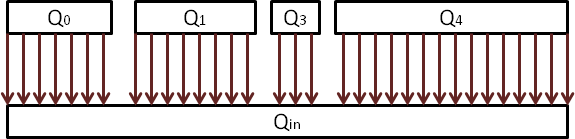
\includegraphics[width=\textwidth,height=0.15\textheight,keepaspectratio]{combine.png}
        \end{enumerate}
    }

    %TODO: this is the worst slide!!!
    \frame{\frametitle{TBN-BFS - Reduce Search Space}
        \begin{enumerate}
            \item $N \gets \size{OutDegrees}$
            \item Each core $i$
                \begin{enumerate}
                    \item $FirstDegree \gets OutDegrees[\floor{\frac{iN}{p}}-1]$
                    \item $FirstDegreeNext \gets OutDegrees[\floor{\frac{(i+1)N}{p}}-1]$
                    \item $FirstCore \gets \ceil{\frac{p~ FirstDegree}{m_\ell}}$
                    \item $LastCore \gets \ceil{\frac{p~ FirstDegreeNext}{m_\ell}}$
                    \item parallel for $j \gets FirstCore$ to $LastCore$
                    \item \T $SubList_j \gets i$
                \end{enumerate}
            \item Using $SubList_i$, core $i$ can search only $n_\ell/p$ indexes
            \item $W_p$ reduces from $\Oh{\size{\V}+\size{\E}+DP\log p}$ to $\Oh{\size{\V}+\size{\E}+DP}$
        \end{enumerate}
    }

    \frame{\frametitle{TBN-BFS - Dynamically Choose Number of Cores}
        \begin{itemize}
            \item In ``Prepare to Split Work'', right after the parallel prefix sum, $p_\ell \gets \func{min}{m_\ell, p}$
            \item Use at most $p_\ell$ cores until next time $m_\ell$ is calculated
            \item This ensures the $\Oh{p_\ell}$ work every level is $\Oh{m_\ell}$
            \item $W_p$ reduces from $\Oh{\size{\V}+\size{\E}+DP}$ to $\Oh{\size{\V}+\size{\E}+D}=\Oh{\size{\V}+\size{\E}}$ (optimal)

                \bigskip
                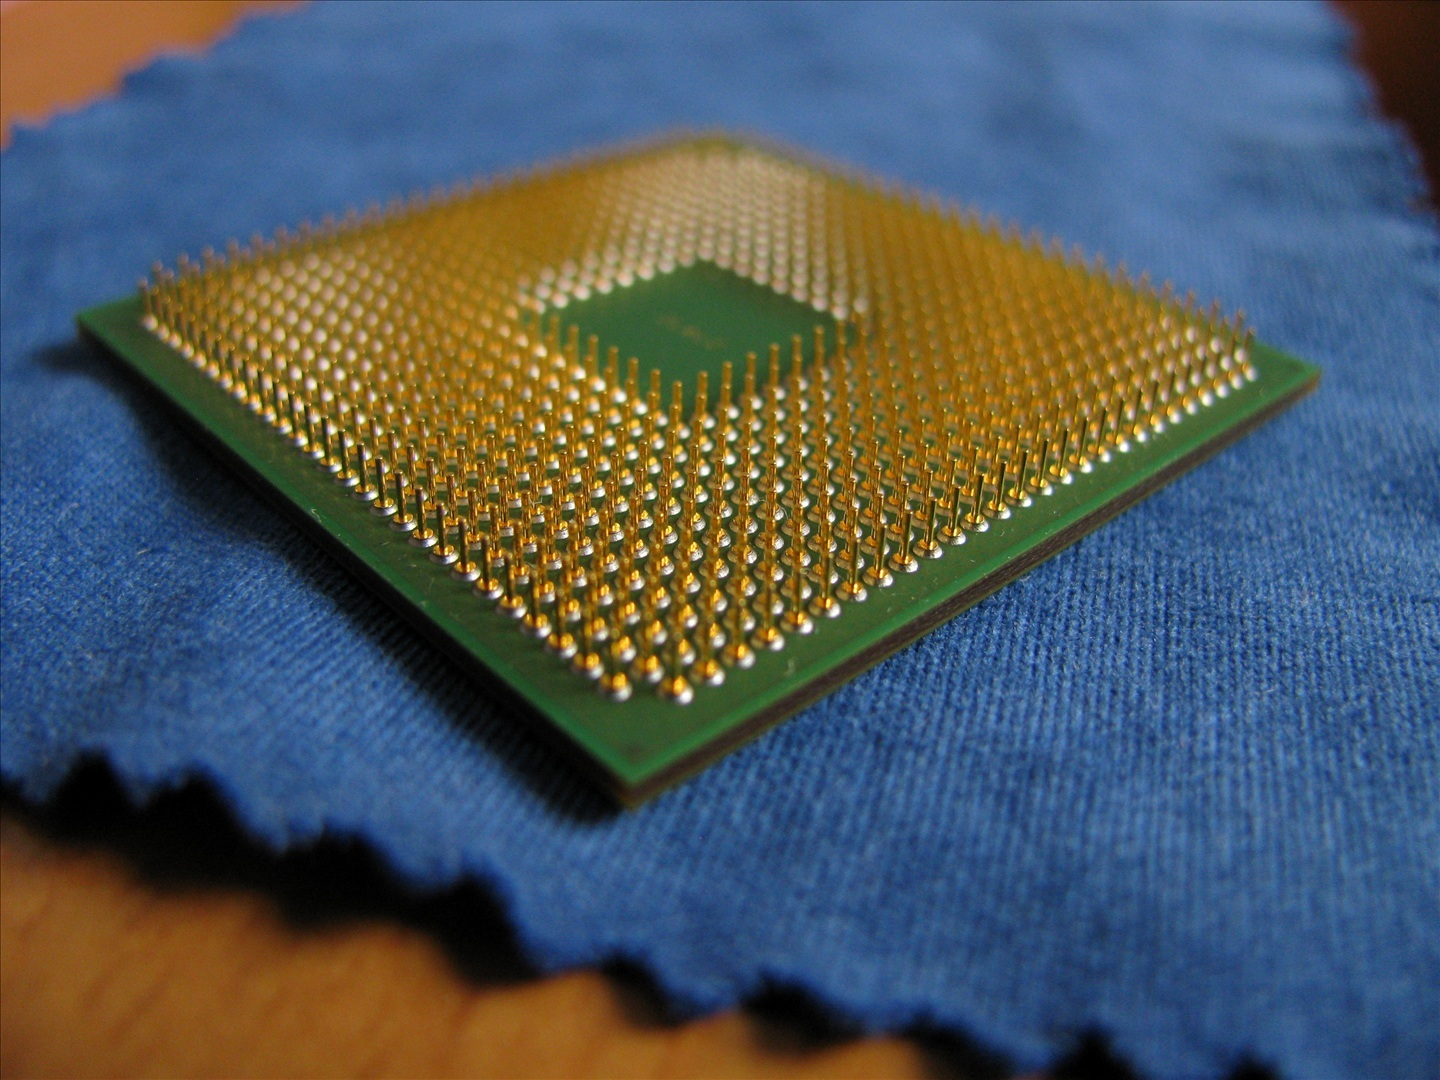
\includegraphics[width=\textwidth,height=0.25\textheight,keepaspectratio]{cpu.jpg}
        \end{itemize}
    }

    %TODO: Conclusion is just ~copy of summary and badly named?
    \frame{\frametitle{Conclusion}
        \begin{itemize}
            \item Our new TBN-BFS algorithm
                \begin{itemize}
                    \item $T_1 = \Oh{\size{\V}+\size{\E}}$ (optimal)
                    \item $W_p = \Oh{\size{\V}+\size{\E}}$ (optimal)
                    \item $T_p = \Oh{\frac{\size{\V}+\size{\E}}{p}+D\log p}$ (optimal)
                    \item Scale-free
                    \item Runs on standard hardware implemented using Cilk+
                    \item Can do its own scheduling deterministically
                    \item Preliminary experiments show merit
                \end{itemize}

                \bigskip
                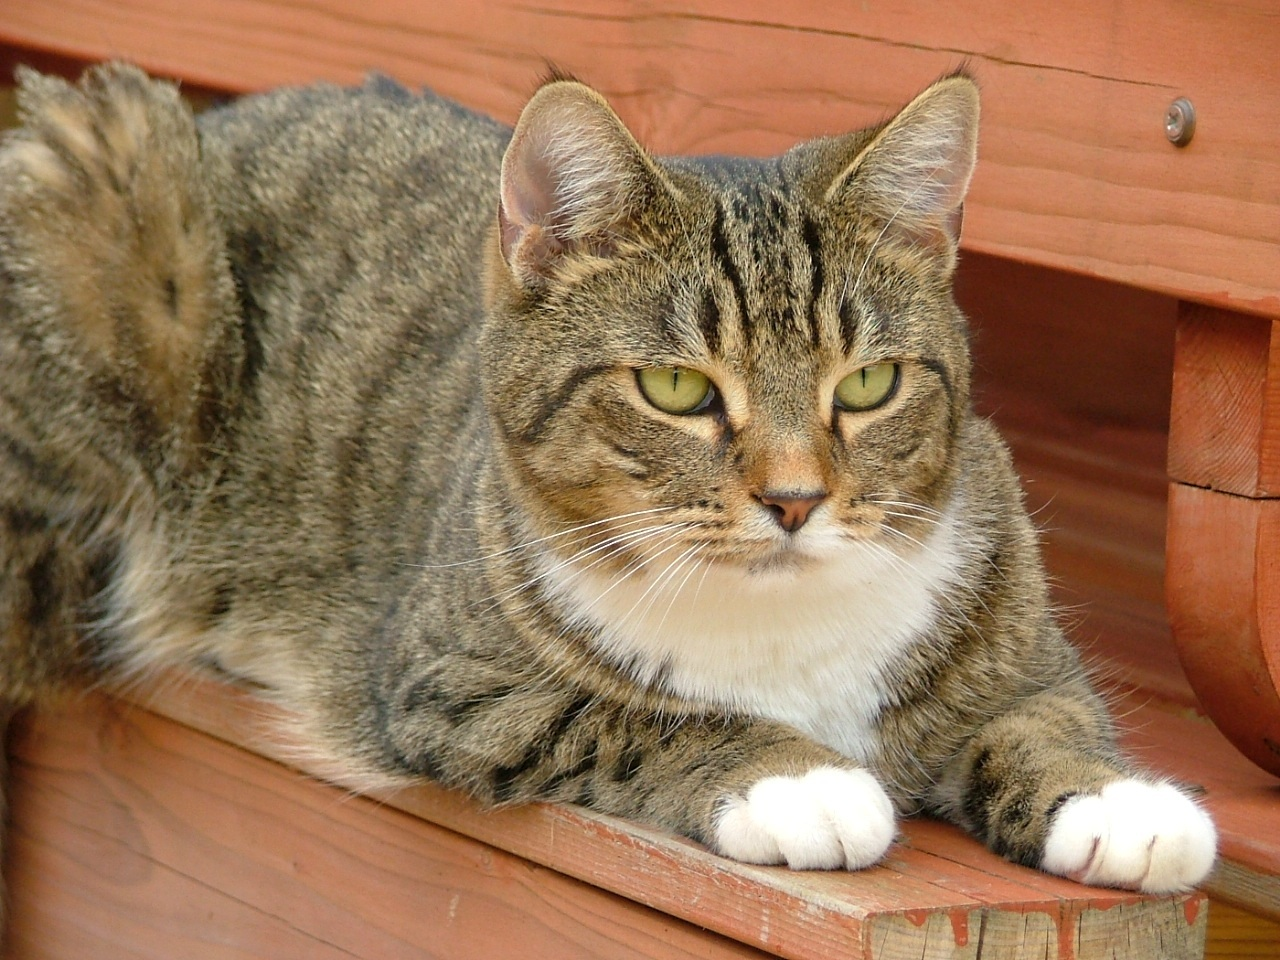
\includegraphics[width=\textwidth,height=0.25\textheight,keepaspectratio]{cat.jpg}
        \end{itemize}
    }

    \frame{\frametitle{Future Work}
        \begin{itemize}
            \item Optimize TBN-BFS for the PRAM model
                \begin{itemize}
                    \item TBN-BFS runs in same time for PRAM but is not asymptotically optimal
                    \item Try using approximate parallel prefix sum \cite{Goldberg95optimaldeterministic}
                \end{itemize}
            \item Modify TBN-BFS to remove false sharing
                \begin{itemize}
                    \item Examine using an $\Oh{n}$ sort algorithm for levels where $m_\ell = \Om{n^\frac{1}{c}}$
                    \item Try to distribute work by cacheline
                \end{itemize}
            \item Examine non level-synchronous approaches
            \item Implement and optimize TBN-BFS
            \item Run experiments comparing TBN-BFS to existing algorithms
        \end{itemize}
    }

    \begin{frame}[allowframebreaks]
        \frametitle{References}
    %\bibliographystyle{amsalpha}
        \bibliographystyle{apalike}
        \bibliography{../source/bib/paper.bib}
    \end{frame}

    \end{document}






%TODO:
    Add figures/slides/references for:


    False sharing
    CILK+

    Related work
    m




































    \iffalse
%\subsection{Subsection no.1.1  }
%\frame{
%Without title somethink is missing.
%}


    \section{Section no. 2}
    \subsection{Lists I}
    \frame{\frametitle{unnumbered lists}
        \begin{itemize}
            \item Introduction to  \LaTeX
            \item Course 2
            \item Termpapers and presentations with \LaTeX
            \item Beamer class
        \end{itemize}
    }

    \frame{\frametitle{lists with maybepause}
        \begin{itemize}
            \item Introduction to  \LaTeX \maybepause
            \item Course 2 \maybepause
            \item Termpapers and presentations with \LaTeX \maybepause
            \item Beamer class
        \end{itemize}
    }

    \subsection{Lists II}
    \frame{\frametitle{numbered lists}
        \begin{enumerate}
            \item Introduction to  \LaTeX
            \item Course 2
            \item Termpapers and presentations with \LaTeX
            \item Beamer class
        \end{enumerate}
    }
    \frame{\frametitle{numbered lists with maybepause}
        \begin{enumerate}
            \item Introduction to  \LaTeX \maybepause
            \item Course 2 \maybepause
            \item Termpapers and presentations with \LaTeX \maybepause
            \item Beamer class
        \end{enumerate}
    }

    \section{Section no.3}
    \subsection{Tables}
    \frame{\frametitle{Tables}
        \begin{tabular}{|c|c|c|}
            \hline
            \textbf{Date} & \textbf{Instructor} & \textbf{Title} \\
            \hline
            WS 04/05 & Sascha Frank & First steps with  \LaTeX  \\
            \hline
            SS 05 & Sascha Frank & \LaTeX \ Course serial \\
            \hline
    \end{tabular}}


    \frame{\frametitle{Tables with maybepause}
        \begin{tabular}{c c c}
            A & B & C \\
            \maybepause
            1 & 2 & 3 \\
            \maybepause
            A & B & C \\
    \end{tabular} }


    \section{Section no. 4}
    \subsection{blocs}
    \frame{\frametitle{blocs}

        \begin{block}{title of the bloc}
            bloc text
        \end{block}

        \begin{exampleblock}{title of the bloc}
            bloc text
        \end{exampleblock}


        \begin{alertblock}{title of the bloc}
            bloc text
        \end{alertblock}
    }
    \fi
